\documentclass[11pt,a4paper]{article}
\PassOptionsToPackage{hyphens}{url}

% =====================================================================
%   PAKETLER (Önce paketler yüklenmelidir)
% =====================================================================
\usepackage[utf8]{inputenc}
\usepackage[T1]{fontenc}
\usepackage[a4paper,left=2.7cm,right=2.7cm,top=2.8cm,bottom=2.8cm,headsep=12pt,headheight=14pt]{geometry}
\IfFileExists{lmodern.sty}{\usepackage{lmodern}}{}
\IfFileExists{lmodern.sty}{\usepackage{microtype}}{\usepackage[expansion=false]{microtype}}

\usepackage{etoolbox}
\usepackage{graphicx}
\usepackage{xcolor}
\usepackage{titlesec}
\usepackage{titling}
\usepackage{fancyhdr}
\usepackage{enumitem}
\usepackage{booktabs}
\usepackage{array}
\usepackage{caption}
\usepackage{subcaption}
\usepackage{amsmath,amssymb}
\usepackage{listings}
\usepackage{tcolorbox}
\tcbuselibrary{skins,breakable}
\usepackage[hidelinks]{hyperref}
\usepackage[capitalise]{cleveref}
\usepackage{csquotes}
\usepackage{setspace}
\usepackage{tabularx}
\usepackage{multirow}
\usepackage{float}
\usepackage{tikz}
\usetikzlibrary{positioning,arrows.meta}
\usepackage[numbers,sort&compress]{natbib}
\setlength{\emergencystretch}{2em}

\usepackage[shorthands=off,turkish,english]{babel}

% =====================================================================
%   KONTROL BAYRAĞI / CONTROL FLAG
% =====================================================================
%   DİL VE DERS BAYRAĞI:
%     1 = Türkçe kapak / üst bilgi / başlıklar ve BLM3010 -- Bilgisayar Projesi
%     0 = İngilizce kapak / üst bilgi / başlıklar ve BLM9000 -- Bitirme Çalışması
%    Aşağıdaki DILBAYRAGI{1} kısmını dersinize göre 0 ya da 1 olarak derse göre seçiniz
% -------------------------------------------------------------
\def\DILBAYRAGI{0}

\newtoggle{TURKCE}
\newtoggle{BLMUC}

\ifnum\DILBAYRAGI=1
  \toggletrue{TURKCE}
  \togglefalse{BLMUC}
  \selectlanguage{turkish}
\else
  \togglefalse{TURKCE}
  \togglefalse{BLMUC}
  \selectlanguage{english}
\fi

% --- Dil bayrağına göre İçindekiler / Şekil / Tablo başlıkları ---
\iftoggle{TURKCE}{
  \renewcommand{\contentsname}{İçindekiler}
  \renewcommand{\listfigurename}{Şekiller}
  \renewcommand{\listtablename}{Tablolar}
  \renewcommand{\figurename}{Şekil}
  \renewcommand{\tablename}{Tablo}
}{
  \renewcommand{\contentsname}{Contents}
  \renewcommand{\listfigurename}{List of Figures}
  \renewcommand{\listtablename}{List of Tables}
  \renewcommand{\figurename}{Figure}
  \renewcommand{\tablename}{Table}
}

% =====================================================================
%   RENK PALETİ
% =====================================================================
\definecolor{anacolor}{RGB}{0,0,0}
\definecolor{vurgucolor}{RGB}{0,0,0}
\definecolor{acikgri}{RGB}{245,245,245}
\definecolor{kodgri}{RGB}{250,250,250}
\definecolor{cizgi}{RGB}{0,0,0}

% =====================================================================
%   BAŞLIK BİÇİMLERİ
% =====================================================================
\titleformat{\section}
  {\normalfont\Large\bfseries\color{anacolor}}
  {\thesection}{0.6em}{}
  [\vspace{-2pt}{\color{cizgi}\titlerule[1.1pt]}]

\titleformat{\subsection}
  {\normalfont\large\bfseries\color{anacolor!85!black}}
  {\thesubsection}{0.6em}{}

\titleformat{\subsubsection}
  {\normalfont\normalsize\bfseries\color{vurgucolor}}
  {\thesubsubsection}{0.6em}{}

\titlespacing*{\section}{0pt}{22pt}{12pt}
\titlespacing*{\subsection}{0pt}{14pt}{8pt}
\titlespacing*{\subsubsection}{0pt}{10pt}{6pt}

% =====================================================================
%   ÜST / ALT BİLGİ (HEADER / FOOTER)
% =====================================================================
\pagestyle{fancy}
\fancyhf{}
\renewcommand{\headrulewidth}{0.6pt}
\renewcommand{\footrulewidth}{0.3pt}
\fancyhead[L]{\small\color{gray}\projebasligikisa}
\fancyhead[R]{\small\color{gray}\nouppercase{\leftmark}}
\fancyfoot[C]{\small\color{gray}\thepage}

\fancypagestyle{ilksayfa}{
  \fancyhf{}
  \fancyfoot[C]{\small\color{gray}\thepage}
  \renewcommand{\headrulewidth}{0pt}
  \renewcommand{\footrulewidth}{0.3pt}
}

% =====================================================================
%   KOD BLOKLARI (listings)
% =====================================================================
\lstdefinestyle{kodstil}{
  backgroundcolor=\color{kodgri},
  basicstyle=\ttfamily\small,
  keywordstyle=\color{anacolor}\bfseries,
  commentstyle=\color{gray}\itshape,
  stringstyle=\color{vurgucolor},
  numberstyle=\tiny\color{gray},
  numbers=left,
  numbersep=8pt,
  frame=single,
  rulecolor=\color{cizgi},
  framesep=6pt,
  breaklines=true,
  showstringspaces=false,
  tabsize=2,
  captionpos=b
}
\lstset{style=kodstil}

% =====================================================================
%   BİLGİ KUTUSU
% =====================================================================
\newtcolorbox{bilgikutu}[1][]{
  colback=acikgri, colframe=anacolor,
  boxrule=0.6pt, arc=2pt, left=8pt, right=8pt, top=6pt, bottom=6pt,
  fonttitle=\bfseries\color{white}, colbacktitle=anacolor,
  #1
}

% =====================================================================
%   KAPAK SAYFASI METİNLERİ / COVER PAGE TEXT
% =====================================================================
\newcommand{\txtUniversite}{\iftoggle{TURKCE}{YILDIZ TEKNİK ÜNİVERSİTESİ}{YILDIZ TECHNICAL UNIVERSITY}}
\newcommand{\txtFakulte}{\iftoggle{TURKCE}{ELEKTRİK-ELEKTRONİK FAKÜLTESİ}{Faculty of Electrical and Electronics}}
\newcommand{\txtBolum}{\iftoggle{TURKCE}{Bilgisayar Mühendisliği Bölümü}{Department of Computer Engineering}}

\newcommand{\txtRaporTuru}{%
  \iftoggle{BLMUC}{%
    \iftoggle{TURKCE}{BLM3010 -- Bilgisayar Projesi}{BLM3010 -- Computer Project}%
  }{%
    \iftoggle{TURKCE}{BLM9000 -- Bitirme Çalışması}{BLM9000 -- Graduation Thesis}%
  }%
}

\newcommand{\txtOgrenciNo}{\iftoggle{TURKCE}{Öğrenci No}{Student ID}}
\newcommand{\txtDanismanEt}{\iftoggle{TURKCE}{Danışman}{Advisor}}
\newcommand{\txtAyYil}{\iftoggle{TURKCE}{Kasım 2026}{November 2026}}

% =====================================================================
%   BAŞLIK / YAZAR BİLGİLERİ
% =====================================================================
\newcommand{\projebasligikisa}{\txtRaporTuru}

\title{\vspace{-1.2cm}
  {\color{anacolor}\rule{\linewidth}{1.3pt}}\\[10pt]
  {\Huge\bfseries\color{anacolor} AUGMENTED REALITY-SUPPORTED\\[4pt] MOBILE ROBOT GAME}\\[6pt]
  {\color{anacolor}\rule{\linewidth}{1.3pt}}\\[4pt]
  {\normalsize \txtBolum\ -- \txtRaporTuru}
}

\author{
  \large \textbf{İsa Koçan} \\[2pt]
  \small \txtOgrenciNo: 22011056\\[6pt]
  \large \textbf{Bilal Efe Uysal} \\[2pt]
  \small \txtOgrenciNo: 22011031\\[10pt]
  \large \textbf{\txtDanismanEt:} Dr. Öğr. Üyesi Furkan Çakmak \\[14pt]
  \normalsize \txtUniversite \\
  \normalsize \txtFakulte\ -- \txtBolum
}

\date{\normalsize \txtAyYil}

% =====================================================================
%   BELGE BAŞLANGICI
% =====================================================================
\begin{document}

\pagenumbering{gobble}

\begin{titlepage}
\thispagestyle{empty}
\begin{center}
\vspace*{0cm}


\includegraphics[width=3.5cm]{assets/logo.png}\\[0.8cm]

{\large \txtUniversite}\\[2pt]
{\large \txtFakulte}\\[2pt]
{\large \txtBolum}\\[1.2cm]

{\color{anacolor}\rule{0.85\linewidth}{1.4pt}}\\[14pt]
{\LARGE\bfseries\color{anacolor} AUGMENTED REALITY-SUPPORTED\\[4pt] MOBILE ROBOT GAME}\\[14pt]
{\color{anacolor}\rule{0.85\linewidth}{1.4pt}}\\[1.1cm]

{\Large \txtRaporTuru}\\[1.2cm]

\begin{tabular}{c}
\large \textbf{Bilal Efe Uysal} \\
\small \txtOgrenciNo: 22011031 \\[6pt]
\large \textbf{İsa Koçan} \\
\small \txtOgrenciNo: 22011056
\end{tabular}\\[1cm]

\begin{tabular}{c}
\large \textbf{\txtDanismanEt} \\
Asst. Prof. Dr. Furkan Çakmak
\end{tabular}

\vfill

{\normalsize \txtAyYil}\\[0.4cm]

\end{center}
\end{titlepage}

\pagenumbering{roman}
\setcounter{page}{2}

% ---------------- ÖNSÖZ ----------------
\section*{Preface}
\addcontentsline{toc}{section}{Preface}
Fields such as artificial intelligence, image processing and augmented reality are entering our daily lives rapidly, and systems that combine the physical and digital worlds attract great interest both scientifically and as entertainment. This work grew out of the idea of a game in which a physical robot is driven from a phone and the environment it sees is enriched with virtual objects. Our aim was to build a system from end to end, from hardware to software and from video streaming to finding the robot's position, and to turn it into an experience that anyone can play easily. The work brings together very different areas such as artificial intelligence and image processing, embedded systems, communication and game development in a single system.

We learned new things in many areas during the work. While working on the mechanical and electronic structure of the robot, we met the limits of hardware in the real world. We gained experience in low-latency video streaming, wireless communication and safe driving. The studies we read on artificial intelligence and image processing, localization and game development gave us new perspectives. Beyond that, as a team we learned to divide the work, to combine different ideas and to move toward a common goal.

We sincerely thank our advisor, Asst. Prof. Dr. Furkan Çakmak, who guided us throughout this process. Our advisor's contribution was decisive in building the robot. He provided all the parts, guided us with his knowledge and experience during assembly and supported us with his suggestions whenever we ran into problems. We are deeply grateful to him for sharing his knowledge and experience with us without hesitation and for the support he gave to our work.

We would like to express our sincere thanks to our families, who have always supported us, believed in us and been patient with us throughout our education and this work. We also thank our friends, who took the time to help with our experiments and stood by us with their ideas and support. We could not have brought this work to this point without them.

While preparing this work, we remember with respect, gratitude and longing Gazi Mustafa Kemal Atatürk, the founder of our Republic, who regarded reason and science as the true guide. The value he gave to education and science, with the aim of raising our country above the level of contemporary civilization, is a guide for young engineering candidates like us. If we can study at a university and carry out scientific work today, we owe it to the Republic he founded and to everyone who has worked toward this goal. We consider it our duty to keep working, producing and being useful to our country in line with the goals he showed us.

\vspace{1.2cm}
\noindent\hfill Bilal Efe Uysal, İsa Koçan\\
\hspace*{\fill}Kasım 2026

\newpage

% ---------------- ÖZET VE ABSTRACT ----------------
\section*{Özet}
\addcontentsline{toc}{section}{Özet}
Bu bölüm daha sonra doldurulacaktır.

\vspace{1cm}

\section*{Abstract}
\addcontentsline{toc}{section}{Abstract}
This section will be completed later.

\newpage
% ---------------- İÇİNDEKİLER ----------------
\selectlanguage{english}
\tableofcontents
\newpage
\listoffigures
\listoftables
\newpage

\pagenumbering{arabic}
\setcounter{page}{1}

% =====================================================================
%   BÖLÜM-1: GİRİŞ
% =====================================================================
\section{Introduction}
\label{sec:giris}
This section describes the aim and scope of the project and then reviews related work.

\subsection{Aim and Scope}
\label{subsec:amac_kapsam}
In augmented reality (AR) games, virtual content is placed over the real environment, but the only thing that moves in the real environment is usually the player. Adding a physical robot to the game enriches the experience, but placing virtual objects in the right spot requires knowing where the robot is in its environment. Low-cost robots, however, usually have no position sensors.

In this project, we are developing an AR game played at home with a robot that carries a 360° camera and is driven from a phone. Our starting point was Mario Kart Live \cite{mariokartlive2020}, which adds virtual elements to the camera view of remote-controlled cars. Instead of racing, we design the game around exploration, like Pokémon GO \cite{paavilainen2017pokemon}. Pokémon GO ties virtual objects to real locations using the global positioning system (GPS). Since GPS is not available indoors, our equivalent is the map of the room and the position of the robot on that map. We do not use a separate sensor on the robot for this and aim to find its position from the 360° camera image alone. We plan to use artificial intelligence and image processing methods for this. The room map is created once and stored, using the light detection and ranging (LiDAR) sensor of an iPhone, or the dual cameras on phones without LiDAR. During play, the robot's 360° image is matched against this map to find the robot's position.

The goals of the project are as follows:
\begin{enumerate}[label=G\arabic*.]
  \item Build a robot that can be driven wirelessly from a phone, streams 360° video with low latency and stops when the connection is lost.
  \item Create the map of the room with LiDAR or dual cameras and store it.
  \item Track the robot's position by matching the 360° image with this map.
  \item Develop a playable AR game that depends on the robot's position.
\end{enumerate}
Our scope is indoor spaces such as a home and single-player use. The application is being developed with Unity and will run on Android and iOS.

\subsection{Literature Review}
\label{subsec:literatur}
Related work is reviewed under four headings, and the position of the project among these studies is stated.

\paragraph{AR and robot games.}
Azuma \cite{azuma1997survey} defined AR as systems that combine real and virtual content, allow real-time interaction and align virtual objects with the real world in three dimensions, and identified registration errors as a core problem. A study on Pokémon GO showed that players see exploring the real world as one of the good sides of the game \cite{paavilainen2017pokemon}. Pratticò and Lamberti \cite{prattico2021mixed} argued that mixed reality games that combine robots with digital elements can overcome the limited game options of consumer robots. In the commercial example Mario Kart Live \cite{mariokartlive2020}, the play area is defined by physical gate markers placed in the room. This product was introduced through a press release, so it is not an academic source.

\paragraph{Room scanning with phones.}
Luetzenburg et al. \cite{luetzenburg2021iphone} showed that the LiDAR sensors of the iPhone 12 Pro and iPad Pro can produce models with an accuracy of about $\pm$1~cm for small objects and about $\pm$10~cm for areas up to 130~m long. Apple's ARKit library can extract the environment as a polygon mesh on LiDAR-equipped devices \cite{apple2026arkit}. On phones without LiDAR, learning-based depth estimation that combines the main and telephoto cameras can be used \cite{zhang2020dunet}.

\paragraph{Camera localization in a known map.}
PICCOLO finds the position of a single 360° panorama inside a colored point cloud without any training \cite{kim2021piccolo}. CPO continues to work even if the scene changes after the map is created \cite{kim2022cpo}, which matters in homes where objects often move. Monte Carlo localization can be used to track position estimates over time \cite{dellaert1999mcl}. A visual odometry study that achieved a position error of 0.21\% over about 17~m with a single downward-looking camera also shows that finding position from a camera alone is possible \cite{patruno2020visual}.

\paragraph{Remote driving with a 360° camera.}
A recent survey on low-latency video streaming lists remote driving among the applications that need low latency \cite{tang2026lowlatency}. In a telepresence robot, a 360° camera gave a stronger sense of presence but left environmental awareness lacking \cite{heshmat2018geocaching}. These findings show that streaming the robot's 360° video to the phone with low latency is critical for the game experience.

\paragraph{Position of the project in the literature.}
The reviewed studies are summarized in Table~\ref{tab:literatur_karsilastirma}. Location-based AR games rely on the player's own movement, and robot games rely on external markers. Methods that localize a panorama inside a map have not been tried in a game context or on a low-cost robot. Our project combines creating the room map with the player's phone, finding the robot's position with the 360° camera alone and without extra sensors, and using this in a game.

\begin{table}[H]
\centering
\caption{Comparison of the reviewed studies}
\label{tab:literatur_karsilastirma}
\small
\begin{tabularx}{\linewidth}{>{\raggedright\arraybackslash}X c c c >{\raggedright\arraybackslash}X c}
\toprule
\textbf{Study} & \textbf{Robot} & \textbf{360° camera} & \textbf{AR} & \textbf{Link to the real space} & \textbf{Game} \\
\midrule
Pokémon GO \cite{paavilainen2017pokemon} & -- & -- & \checkmark & Phone location & \checkmark \\
Mario Kart Live \cite{mariokartlive2020} & \checkmark & -- & \checkmark & Physical gate markers & \checkmark \\
Heshmat et al. \cite{heshmat2018geocaching} & \checkmark & \checkmark & -- & -- & -- \\
Patruno et al. \cite{patruno2020visual} & \checkmark & -- & -- & Relative position from a downward-looking camera & -- \\
PICCOLO / CPO \cite{kim2021piccolo,kim2022cpo} & -- & \checkmark & -- & Pre-scanned point cloud & -- \\
This project & \checkmark & \checkmark & \checkmark & Room map scanned with a phone & \checkmark \\
\bottomrule
\end{tabularx}
\end{table}

The rest of the report is organized as follows. Section~\ref{sec:analiz_fizibilite} presents the system analysis and feasibility. System design, experimental results, and conclusion and discussion will be presented in later stages.

% =====================================================================
%   SECTION 2: SYSTEM ANALYSIS AND FEASIBILITY
% =====================================================================
\newpage
\section{System Analysis and Feasibility}
\label{sec:analiz_fizibilite}
This section identifies the components, requirements and constraints of the system and then evaluates the feasibility of the project in terms of software, hardware and time.

\subsection{System Analysis}
\label{subsec:sistem_analizi}
The system consists of a Unity game application running on the phone and a 360° camera robot driven wirelessly from it (Figure~\ref{fig:sistem_bilesenleri}). The robot computer (NVIDIA Jetson Nano) forwards the video of the 360° camera (Ricoh Theta S), which is connected with a universal serial bus (USB) cable, to the phone and passes driving commands to the microcontroller (Arduino Uno). The microcontroller controls the direct current (DC) motors, the light emitting diode (LED) and the buzzer. The player scans the room once with a LiDAR-equipped phone. While the player drives the robot, the application finds the robot's position on the map and places virtual objects accordingly (Figure~\ref{fig:konum_akisi}).

\begin{figure}[H]
\centering
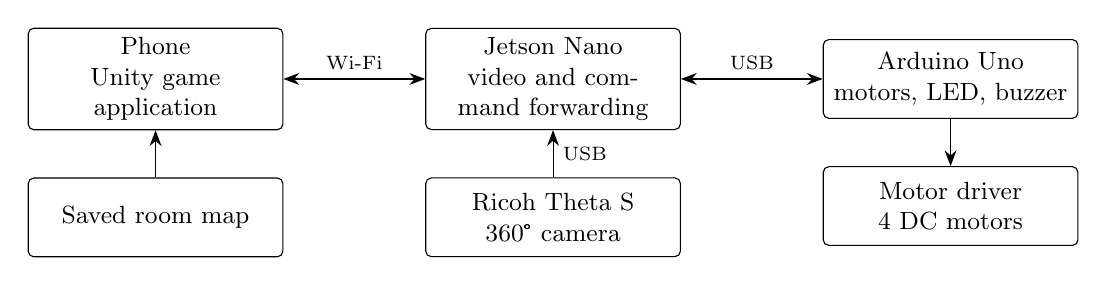
\begin{tikzpicture}[
  box/.style={draw, rounded corners=2pt, minimum height=1cm, text width=3cm, align=center, font=\small},
  >={Stealth[length=2mm]}]
\node[box] (tel) {Phone\\Unity game application};
\node[box, right=1.8cm of tel] (jet) {Jetson Nano\\video and command forwarding};
\node[box, right=1.8cm of jet] (ard) {Arduino Uno\\motors, LED, buzzer};
\node[box, below=0.6cm of tel] (harita) {Saved room map};
\node[box, below=0.6cm of jet] (cam) {Ricoh Theta S\\360° camera};
\node[box, below=0.6cm of ard] (mot) {Motor driver\\4 DC motors};
\draw[<->] (tel) -- node[above, font=\scriptsize]{Wi-Fi} (jet);
\draw[<->] (jet) -- node[above, font=\scriptsize]{USB} (ard);
\draw[->] (cam) -- node[right, font=\scriptsize]{USB} (jet);
\draw[->] (ard) -- (mot);
\draw[->] (harita) -- (tel);
\end{tikzpicture}
\caption{Components of the system and the connections between them}
\label{fig:sistem_bilesenleri}
\end{figure}

\begin{figure}[H]
\centering
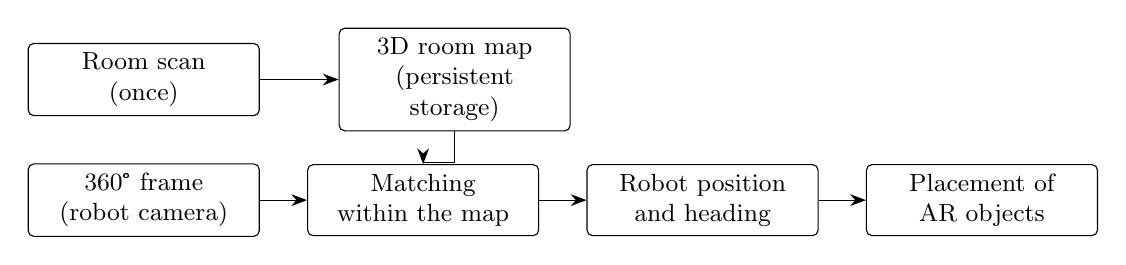
\begin{tikzpicture}[
  box/.style={draw, rounded corners=2pt, minimum height=0.9cm, text width=2.7cm, align=center, font=\small},
  >={Stealth[length=2mm]}]
\node[box] (tara) {Room scan\\(once)};
\node[box, right=1cm of tara] (harita) {3D room map\\(persistent storage)};
\node[box, below=0.6cm of tara] (kare) {360° frame\\(robot camera)};
\node[box, right=0.6cm of kare] (esle) {Matching within the map};
\node[box, right=0.6cm of esle] (konum) {Robot position and heading};
\node[box, right=0.6cm of konum] (ar) {Placement of AR objects};
\draw[->] (tara) -- (harita);
\draw[->] (harita.south) -- ++(0,-0.4) -| (esle.north);
\draw[->] (kare) -- (esle);
\draw[->] (esle) -- (konum);
\draw[->] (konum) -- (ar);
\end{tikzpicture}
\caption{Proposed localization flow}
\label{fig:konum_akisi}
\end{figure}

\paragraph{Requirements and constraints.}
The functional (FR) and non-functional (NFR) requirements are given in Table~\ref{tab:gereksinimler}. The robot has no position sensor, and because the wheels slip in skid-steer driving, its position must be found from the camera. The height difference between the room scan and the robot camera may make matching harder, and LiDAR exists only on some devices and has a limited range \cite{luetzenburg2021iphone}.

\begin{table}[!ht]
\centering
\caption{Requirements of the system}
\label{tab:gereksinimler}
\small
\begin{tabularx}{\linewidth}{l >{\raggedright\arraybackslash}X}
\toprule
\textbf{Code} & \textbf{Requirement} \\
\midrule
FR-1 & The application must find the robot on the network and connect to it automatically, and the player must be able to drive it and look around in the 360° view. \\
FR-2 & The room map must be created with LiDAR or dual cameras and stored. \\
FR-3 & The robot's position must be tracked within the map, and virtual objects must be placed correctly by detecting the floor and objects. \\
FR-4 & The light (LED) and sound (buzzer) outputs must be used to improve the driving experience, and the player's progress must be saved. \\
NFR-1 & The robot must stop by itself within a short time when the connection is lost. \\
NFR-2 & The video latency must be low enough not to disturb driving \cite{tang2026lowlatency}. \\
NFR-3 & The application must not require technical knowledge and must run on Android and iOS. \\
\bottomrule
\end{tabularx}
\end{table}

\paragraph{Inputs, outputs and metrics.}
The inputs are driving commands, depth data and the 360° video, and the outputs are the room map, the robot's position, the AR view and the commands sent to the robot. Performance will be measured by the position error (cm), the video latency (ms), the number of connection drops and the play time on a full battery (minutes), and the game experience will also be evaluated by letting participants play the game and collecting ratings from them on a scale of 10.

\subsection{Feasibility}
\label{subsec:fizibilite}
The feasibility of the project has been evaluated in terms of software, hardware and time.

\subsubsection{Software Feasibility}
\label{subsubsec:yazilim_fizibilitesi}
The software used is given in Table~\ref{tab:yazilim_araclari}. All of it is free and most of it is open source.

\begin{table}[H]
\centering
\caption{Software used in the project}
\label{tab:yazilim_araclari}
\small
\begin{tabularx}{\linewidth}{>{\raggedright\arraybackslash}p{2.9cm} >{\raggedright\arraybackslash}p{5cm} >{\raggedright\arraybackslash}X}
\toprule
\textbf{Purpose} & \textbf{Tool} & \textbf{Rationale} \\
\midrule
Game and AR & Unity 6.3 LTS, AR Foundation & Builds for Android and iOS from a single code base, widely used in robot-based AR applications \cite{coronado2023integrating} \\
Room scanning & ARKit \cite{apple2026arkit}, dual-camera depth \cite{zhang2020dunet} & Scanning on devices with and without LiDAR \\
Localization & PICCOLO, CPO \cite{kim2021piccolo,kim2022cpo}, PyTorch & Open-source code that finds the position from a panorama and runs on a graphics processor \\
Floor and object detection & Depth Anything \cite{yang2024depthanything}, Segment Anything \cite{kirillov2023sam} & Single-camera depth estimation and segmentation, the smallest version has about 24.8 million parameters \\
Robot and build & JetPack 4.6, GStreamer, Python 3, Arduino IDE, Xcode & Video streaming, robot control and the iOS build \\
\bottomrule
\end{tabularx}
\end{table}

Image processing is likely to run on the robot computer and AR drawing on the phone. This split will be measured in the first experiments and is the highest technical risk of the project. The weights of the smallest Depth Anything version take up roughly 100~MB and fit easily into the 4~GB memory of the robot computer, and its speed will be measured in the first experiments. Because driving, video streaming and the game prototype already work, we find the project feasible in terms of software.

\subsubsection{Hardware Feasibility}
\label{subsubsec:donanim_fizibilitesi}
The parts of the robot and their estimated prices are in Table~\ref{tab:donanim_maliyet}.

\begin{table}[H]
\centering
\caption{Robot and scanning hardware with estimated costs}
\label{tab:donanim_maliyet}
\small
\begin{tabularx}{\linewidth}{>{\raggedright\arraybackslash}X c r}
\toprule
\textbf{Component} & \textbf{Qty} & \textbf{Estimated price (USD)} \\
\midrule
NVIDIA Jetson Nano (4~GB), robot computer & 1 & 99 \\
Arduino Uno Rev3, microcontroller & 1 & 25--30 \\
Pololu Dual VNH5019, DC motor driver & 1 & 70 \\
Ricoh Theta S, 360° camera & 1 & 349 \\
Hsiang Neng HN-GH12-2217Y motor (12~V, 50:1) & 4 & 23 (each) \\
4S lithium polymer (LiPo) battery (14.8~V, 5200~mAh) & 1 & 56--68 \\
Chassis, wheels, relay, buzzer, LED, wiring & -- & 120--170 \\
Apple iPhone 14 Pro, room scanning and game & 1 & 999 \\
\bottomrule
\end{tabularx}

\vspace{2pt}
{\footnotesize Prices are approximate values in United States dollars (USD).}
\end{table}

The connections between the motors, the motor driver, the microcontroller, the robot computer, the 360° camera, the LED and the buzzer have been made, and driving, light, sound and video streaming have been tested and work. We therefore find the project feasible in terms of hardware as well.

\subsubsection{Time Feasibility (Gantt)}
\label{subsubsec:zaman_fizibilitesi}
The project runs for about 13 weeks, between September 28, 2026 and December 28, 2026. The work packages are shown in Table~\ref{tab:gantt}. Dark cells are the work completed up to week 6 (November 2--8, 2026), and light cells are the planned work.

\newcommand{\ganttG}[1][\linewidth]{\textcolor{black!75}{\rule[-0.4ex]{#1}{1.8ex}}}
\newcommand{\ganttP}[1][\linewidth]{\textcolor{black!25}{\rule[-0.4ex]{#1}{1.8ex}}}
\newcolumntype{G}{>{\centering\arraybackslash}p{0.45cm}}

\begin{table}[!ht]
\centering
\caption{Project schedule (Gantt chart)}
\label{tab:gantt}
\small
\setlength{\tabcolsep}{1pt}
\renewcommand{\arraystretch}{1.0}
\begin{tabular}{>{\raggedright\arraybackslash}p{5.8cm} *{13}{G}}
\toprule
 & \multicolumn{5}{c}{\textbf{October}} & \multicolumn{4}{c}{\textbf{November}} & \multicolumn{4}{c}{\textbf{December}} \\
\cmidrule(lr){2-6} \cmidrule(lr){7-10} \cmidrule(lr){11-14}
\textbf{Work package} & 1 & 2 & 3 & 4 & 5 & 6 & 7 & 8 & 9 & 10 & 11 & 12 & 13 \\
\midrule
Planning, design and literature review & \ganttG & \ganttG & \ganttG & \ganttG & \ganttG & \ganttG & \ganttP & \ganttP &  &  &  &  &  \\
Game prototype (simulation) &  & \ganttG & \ganttG & \ganttG & \ganttG &  &  &  &  &  &  &  &  \\
Robot hardware, driving and video streaming &  &  &  & \ganttG & \ganttG & \ganttG & \ganttP &  &  &  &  &  &  \\
Room scanning and localization &  &  &  &  &  &  & \ganttP & \ganttP & \ganttP & \ganttP & \ganttP &  &  \\
Game levels and AR objects &  &  &  &  &  &  &  &  & \ganttP & \ganttP & \ganttP & \ganttP &  \\
Tests and measurements &  &  &  &  &  &  &  &  &  & \ganttP & \ganttP & \ganttP &  \\
Final report and presentation &  &  &  &  &  &  &  &  &  &  &  & \ganttP & \ganttP \\
\bottomrule
\end{tabular}

\vspace{2pt}
{\footnotesize \ganttG[0.45cm]~Completed \qquad \ganttP[0.45cm]~Planned \qquad
Week 1: September 28 -- October 4, 2026, Week 13: December 21 -- 28, 2026}
\end{table}

% Sections 3-5 (System Design, Experimental Results, Conclusion and Discussion) will be written in later reports.
% \newpage
% \section{Sistem Tasarımı / System Design}
% \label{sec:tasarim}
% \subsection{Sistemin Genel Görünümü ve Önerilen Metot / Overview of the System and Proposed Method}
% \subsection{Materyal ve Veri Kümesi / Material and Dataset}
% \subsection{Kullanılan Yöntemler / Methods Used}
% \section{Deneysel Sonuçlar / Experimental Results}
% \section{Sonuç ve Tartışma / Conclusion and Discussion}

% =====================================================================
%   KAYNAKÇA
% =====================================================================
\newpage
\addcontentsline{toc}{section}{References}
\renewcommand{\bibname}{References}
\bibliographystyle{unsrtnat}
\bibliography{kaynaklar_en}

% =====================================================================
%   EKLER
% =====================================================================
\newpage
\appendix
\section{Appendices}
GitHub repository of the work: \url{https://github.com/isakocan/ARrobot}

Video link and QR code: to be added in a later stage.

\end{document}
